\documentclass{beamer}
\mode<presentation>
{
  \usetheme{Madrid}      
  \usecolortheme{seahorse} 
  \usefonttheme{structureitalicserif} 
  \setbeamertemplate{footline}{}
  \setbeamertemplate{caption}[numbered]
} 
\usepackage{tikz}
\setbeamercovered{highly dynamic}

\newcounter{saveenumi}
\newcommand{\seti}{\setcounter{saveenumi}{\value{enumi}}}
\newcommand{\conti}{\setcounter{enumi}{\value{saveenumi}}}
\usetikzlibrary{shapes.geometric,calc,angles,positioning,intersections,quotes,decorations,babel,patterns,fit}
\usepackage{tkz-euclide}
\usetkzobj{all}
\usepackage[english]{babel}
\usepackage[utf8]{inputenc}
\usepackage[T1]{fontenc}
\usepackage{hyperref}
\usepackage{graphics}
\usepackage{hyperref}
\hypersetup{
    colorlinks=true,
    linkcolor=blue,
    filecolor=magenta,      
    urlcolor=cyan,
    pdftitle={Sharelatex Example},
    bookmarks=true,
    pdfpagemode=FullScreen,
}
 
\urlstyle{same}
\graphicspath{ {.//home/lenovo/codes/circle} }
\usepackage{standalone}
\usepackage{gensymb}
\title[Your Short Title]{Excercise}
\author{Pratibha}
\institute{}
\date{3 Jan 2020}

\begin{document}

\begin{frame}
  \titlepage
\end{frame}
\begin{frame}{Miscellaneous Exercises}
\begin{enumerate}
\conti
\item The length of the
minute hand of a clock is 14 cm. Find the area
swept by the minute hand in 5 minutes.\\
\seti
\end{enumerate}
\begin{itemize}
\item \textbf{Solution} :
\item Given r = 14 
\begin{figure}[!ht]
\resizebox{0.5\linewidth}{!}
{
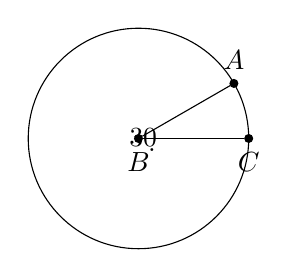
\begin{tikzpicture}
[scale =0.1,>=stealth,point/.style = {draw, circle, fill = black, inner sep = 1pt},]
\node (B) at (0,0)[point,label=below :$B$] {};
\node (C) at (14,0)[point,label=below :$C$] {};
\node (A) at (12.12,6.99)[point,label=above :$A$] {};
\draw (0,0) node [below right] {.} circle (14);
\draw (B)--(A);
\draw (B)--(C);
\tkzMarkAngle[fill=green!40,size=0.1cm,mark=](C,B,A)
\tkzLabelAngle[pos=0.1](C,B,A){\rotatebox{-360}{$30$}}
\end{tikzpicture}


}

\end{figure}


\end{itemize}
\end{frame}
\begin{frame}
\begin{figure}
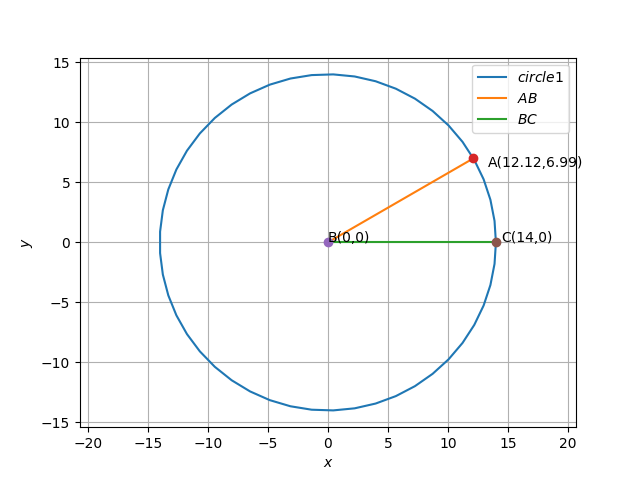
\includegraphics[scale=.6]{./CODES/MISC.png}
\end{figure}
\end{frame}
\begin{frame}

 In 60 minutes minute hand covers  360$\degree$\\
For 5 minutes 6$\degree$ $\times$ 5 = 30$\degree$\\ 
Here $\theta$ = 30 $\degree$ and r = 14cm\\

\begin{align*}
	\text{Area of sector} = \frac{\theta}{360} \times \pi r^2
	=51.31cm^2.
\end{align*}   
\begin{itemize}
\item \url {https://github.com/pratibha444/GEOMETRY/blob/master/CODES/MISC.py} 
\end{itemize}             
\end{frame}
\begin{frame}{Circle construction}

 Construct a tangent to a circle of radius 4 units
from a point on the concentric circle of radius
6 units.\\
\begin{itemize}
\item\textbf{Solution} :\\
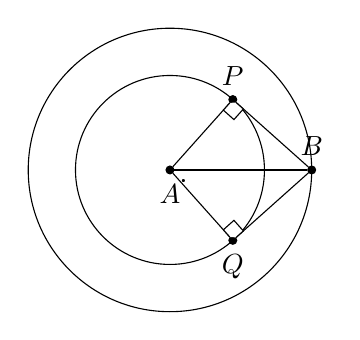
\begin{tikzpicture}
[scale =0.3,>=stealth,point/.style = {draw, circle, fill = black, inner sep = 1pt},]
\node (A) at (0,0)[point,label=below :$A$] {};
\node (P) at (2.66,2.98)[point,label=above :$P$] {};
\node (B) at (6,0)[point,label=above :$B$] {};
\node (Q) at (2.66,-2.98)[point,label=below :$Q$] {};
\draw (0,0) node [below right] {.} circle (6);
\draw (0,0) node [below right] {.} circle (4);
\draw (B)--(A);
\draw (B)--(Q);
\draw (B)--(P);
\draw (A)--(P);
\draw (A)--(Q);
\tkzMarkRightAngle[fill=white!45,size=.6,mark=](B,P,A)
\tkzMarkRightAngle[fill=white!45,size=.6,mark=](B,Q,A)
\end{tikzpicture}
\\  PB and QB are the tangents 
\end{itemize}
\seti
\end{frame}

\begin{frame}
\begin{itemize}
\item \textbf{Given} : r1=4 and r2 = 6\\
\begin{align*}
a=\sqrt{r2^2 - r1^2}\\
a=4.47\\
c=r1 , b=r2\\
p=\frac{b^2+c^2-a^2}{2b}\\
p=2.66\\
q=\sqrt{c^2 - p^2}\\
q=2.98\\
AB = r2 \\
P = (2.66,2.98)\\
Q = (2.66,-2.98)
\end{align*}
\end{itemize}

\end{frame}


\begin{frame}
\begin{figure}
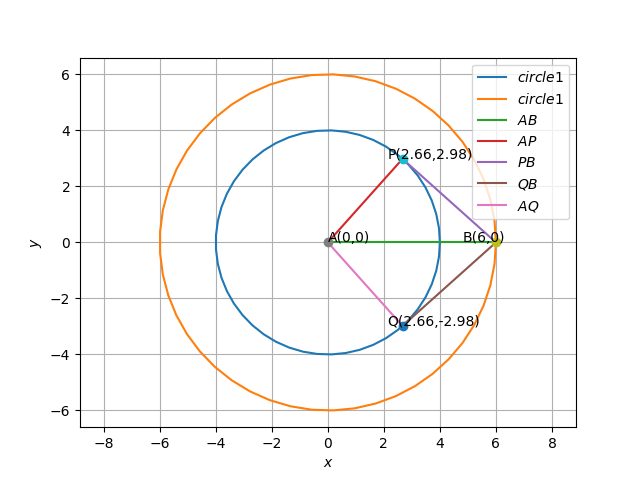
\includegraphics[scale=.4]{./CODES/circle/CIR_CON.png}
\end{figure}
\begin{itemize}
\item \url{https://github.com/pratibha444/GEOMETRY/blob/master/figs/CIRCLE_CON.tex}  \\
\item \url{https://github.com/pratibha444/GEOMETRY/blob/master/CODES/circle/circon.py}
\end{itemize}
\end{frame}

\end{document}